\section{AV平面にプロット}
この節では歌詞をAV平面上にプロットした結果について記述する.

\subsection{楽曲}
楽曲に登場する歌詞のフレーズのAV値の平均を歌詞のAV値とした.図3.2はAV平面に楽曲をプロットした図である.
\begin{figure}[h]
    \centering
    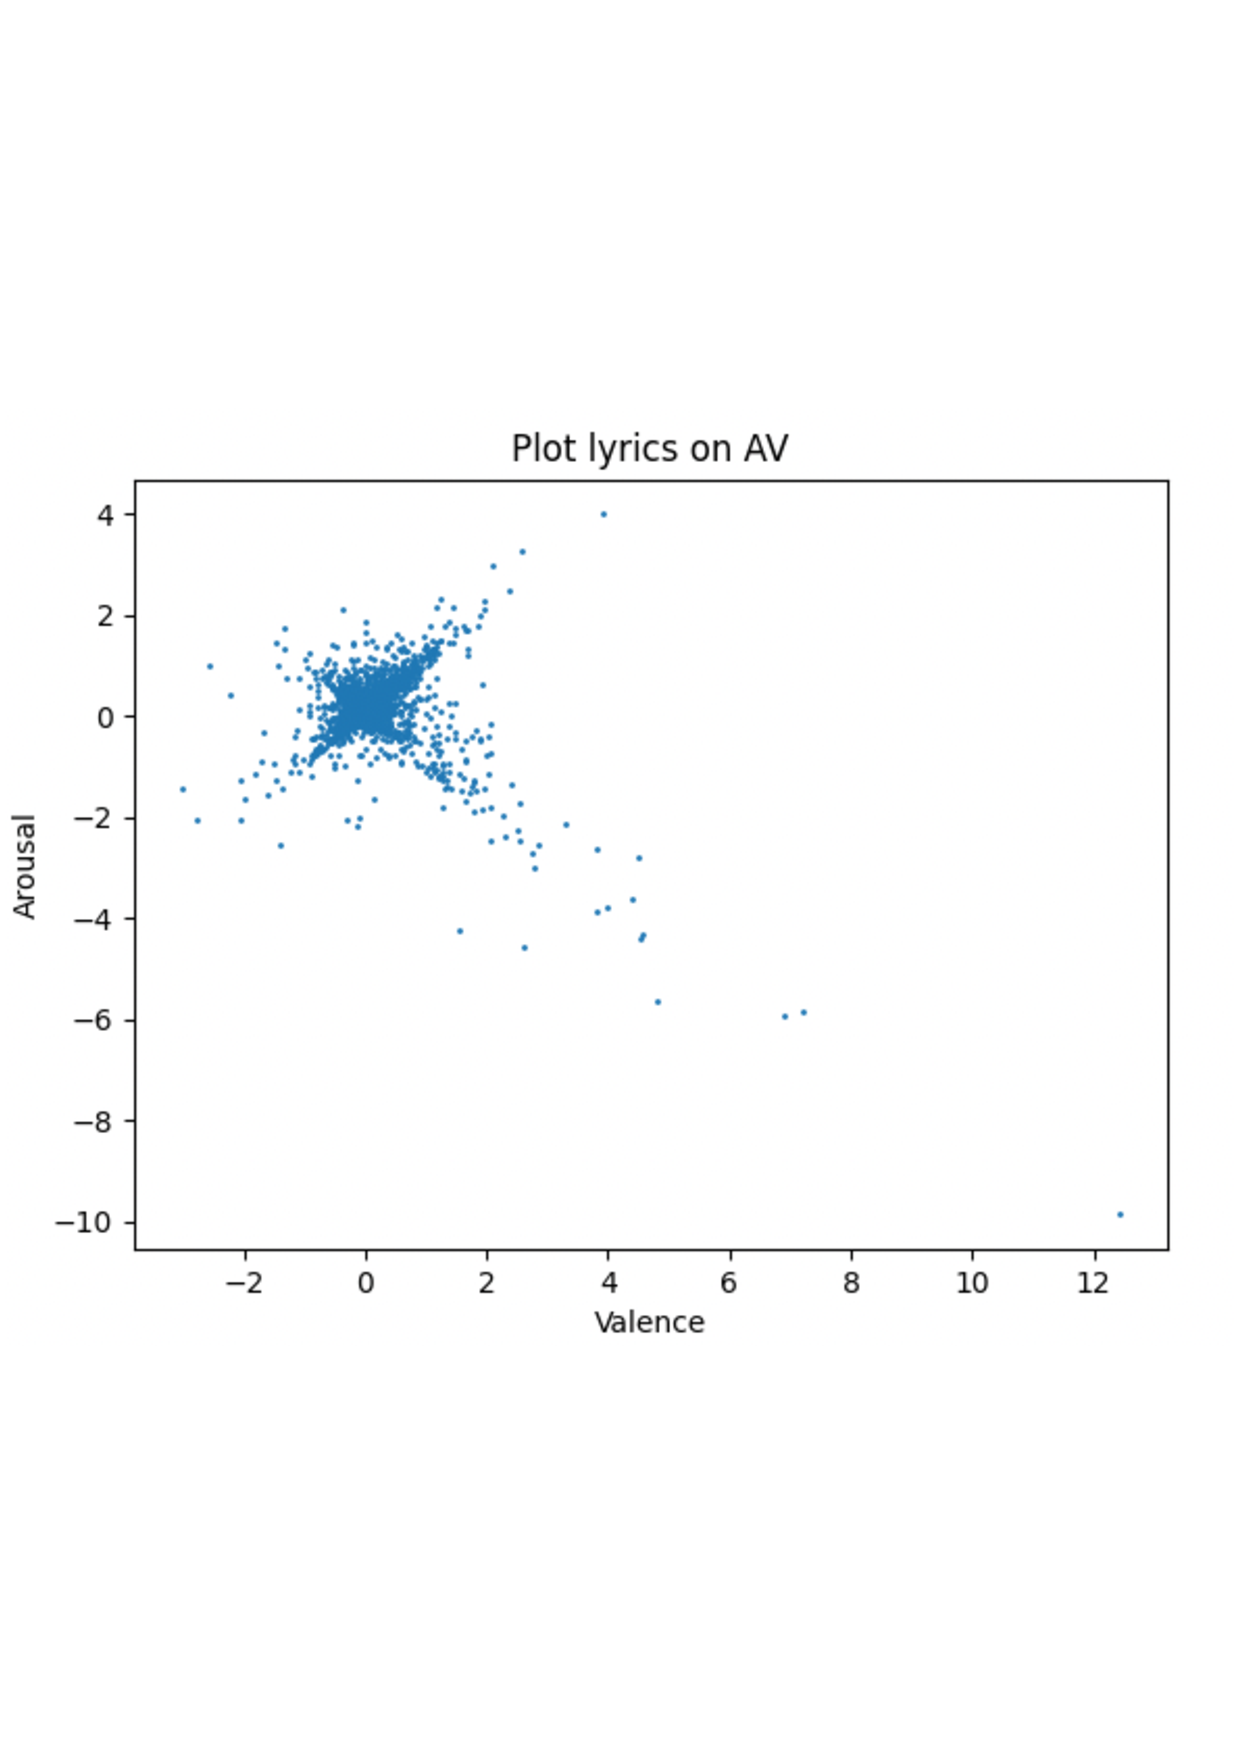
\includegraphics[width=12cm]{lyrics_AV.pdf}
    \vspace{0mm}
    \caption{歌詞 AV平面}
    \label{fig:vkall}
    \vspace{5mm}
\end{figure}

各印象ごとに歌詞を分類して,ward法で原点からの距離に基づいて3グループにクラスタリングした.
薄い肌色でプロットされている原点から一番近いグループを第1グループ.赤紫色でプロットされている原点から2番目に近いグループを第2グループ.黒色でプロットされている原点からもっとも遠いグループを第3グループとする.
\newpage
第1象限のプロット図は図3.3である.
\begin{figure}[H]
  \centering
  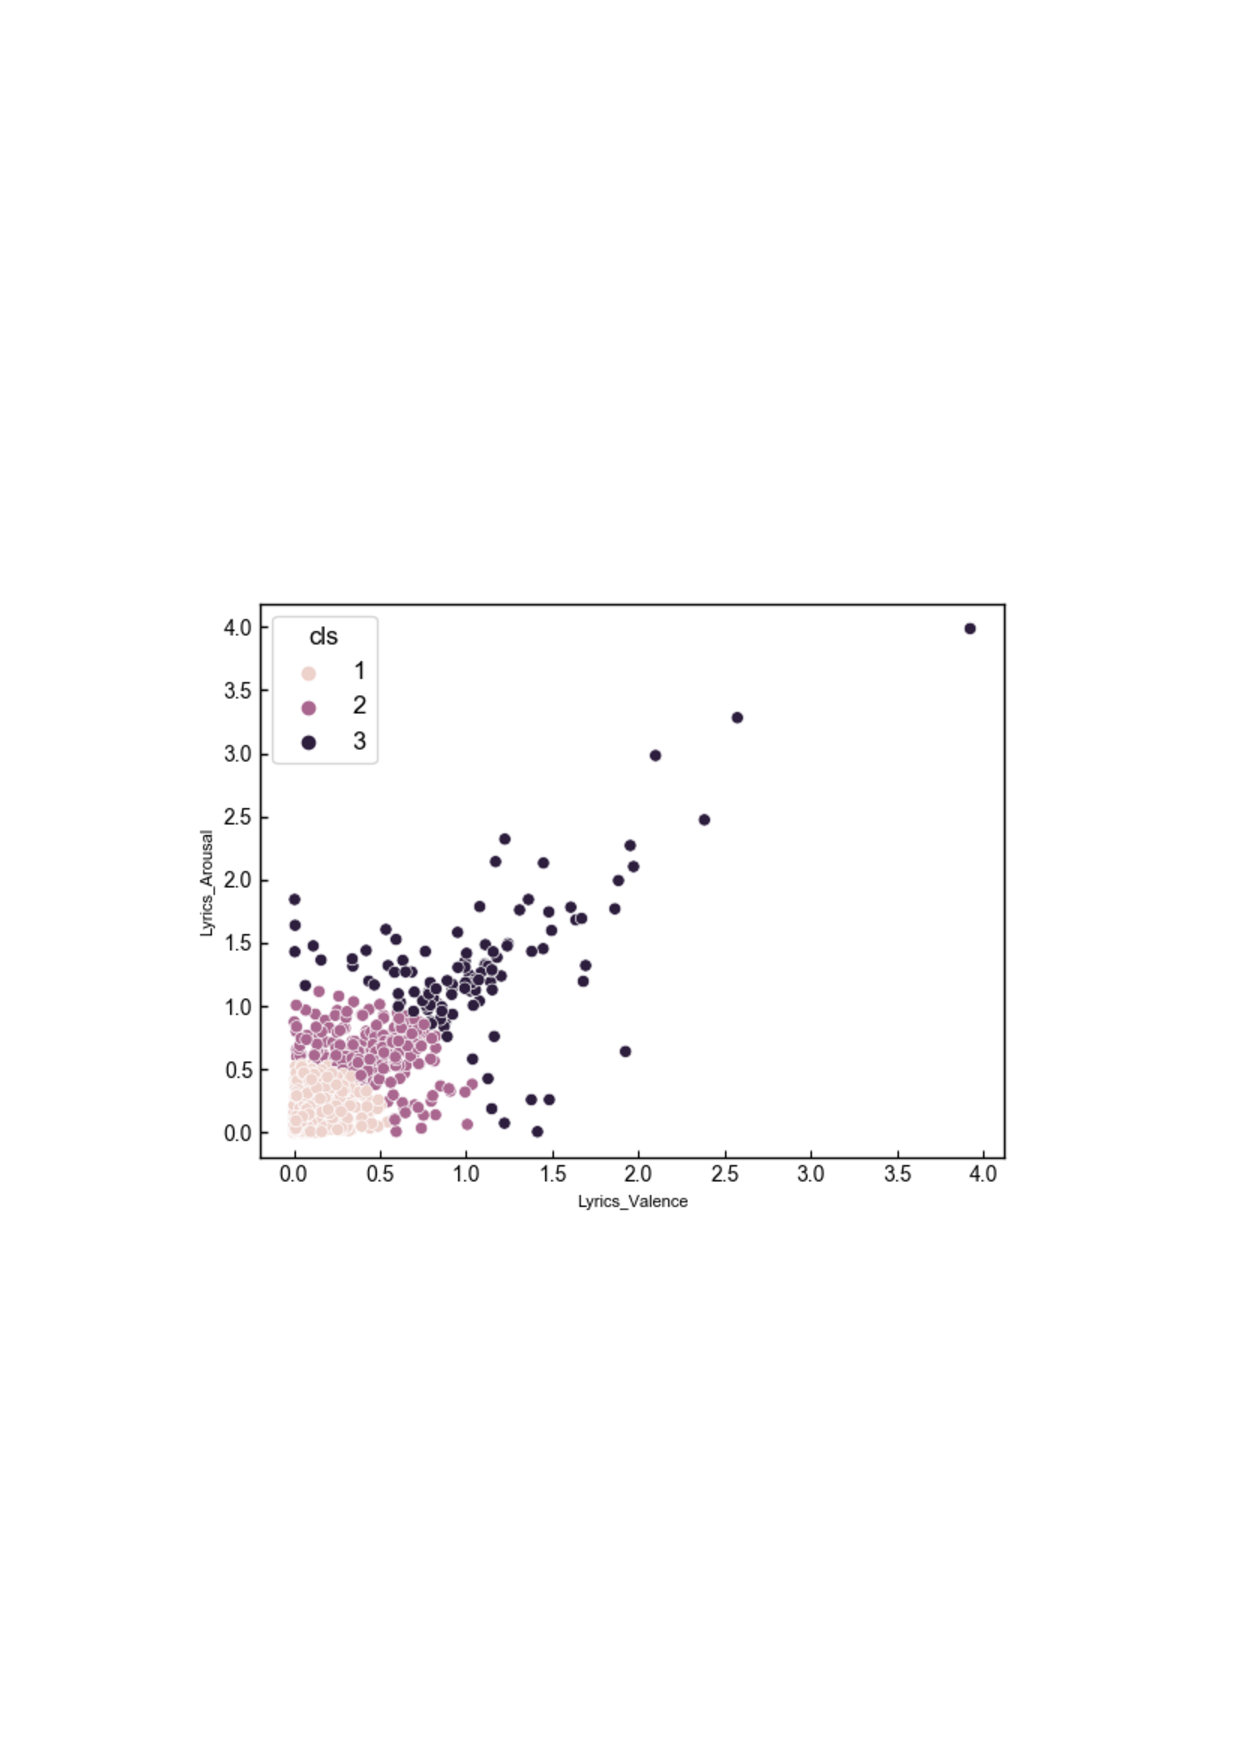
\includegraphics[width=14cm]{lyrics_A+V+.pdf}
  \vspace{-1mm}
  \caption{歌詞 A+V+平面}
  \label{fig:vkall}
  \vspace{5mm}
\end{figure}
第1象限にプロットされた楽曲は全部で1,424曲である.そのうちウォード法によって分割された曲数は第1グループが1015曲,第2グループが296曲,第3グループが112曲であった.
後述する実験に用いる楽曲の歌詞データはそれぞれのグループからランダムで1曲分選出する.
第1グループからはコブクロの「光の誓いが聴こえた日」,第2グループからは椎名林檎の「積み木遊び」,第3グループからはDREAM COME TRUEの「冬三昧にはまだ遠い」の3曲を選出した.
\newpage
第2象限のプロット図は図3.4である.
\begin{figure}[H]
  \centering
  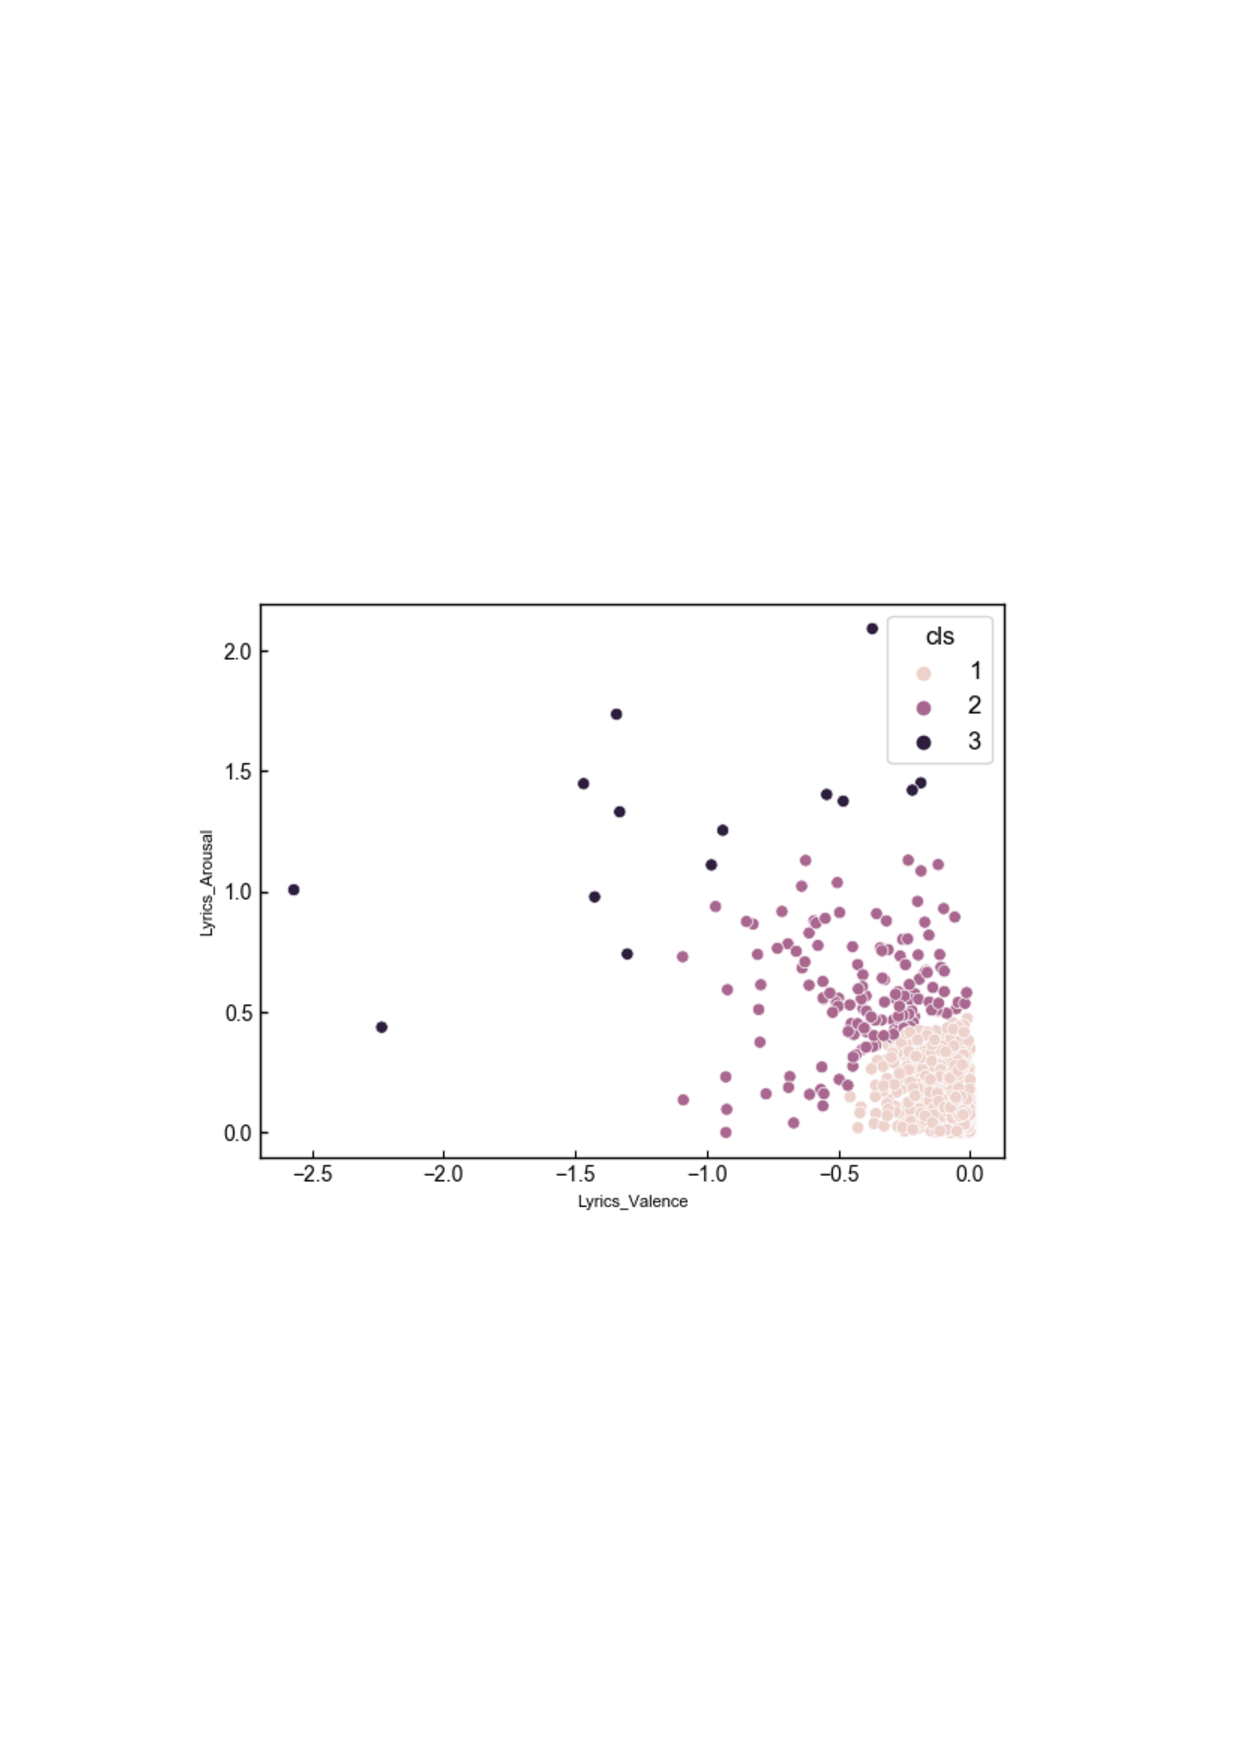
\includegraphics[width=14cm]{lyrics_A+V-.pdf}
  \vspace{-1mm}
  \caption{歌詞 A+V-平面}
  \label{fig:vkall}
  \vspace{5mm}
\end{figure}
第2象限にプロットされた楽曲は全部で887曲である.そのうちウォード法によって分割された曲数は第1グループが728曲,第2グループが145曲,第3グループが14曲であった.
後述する実験に用いる楽曲の歌詞データはそれぞれのグループからランダムで1曲分選出する.
第1グループからは,第2グループからはRADWIMPSの「透明人間18号」,第3グループからはB'zの「Da La Da Da」の3曲を選出した.
\newpage
第3象限のプロット図は図3.5である.
\begin{figure}[H]
  \centering
  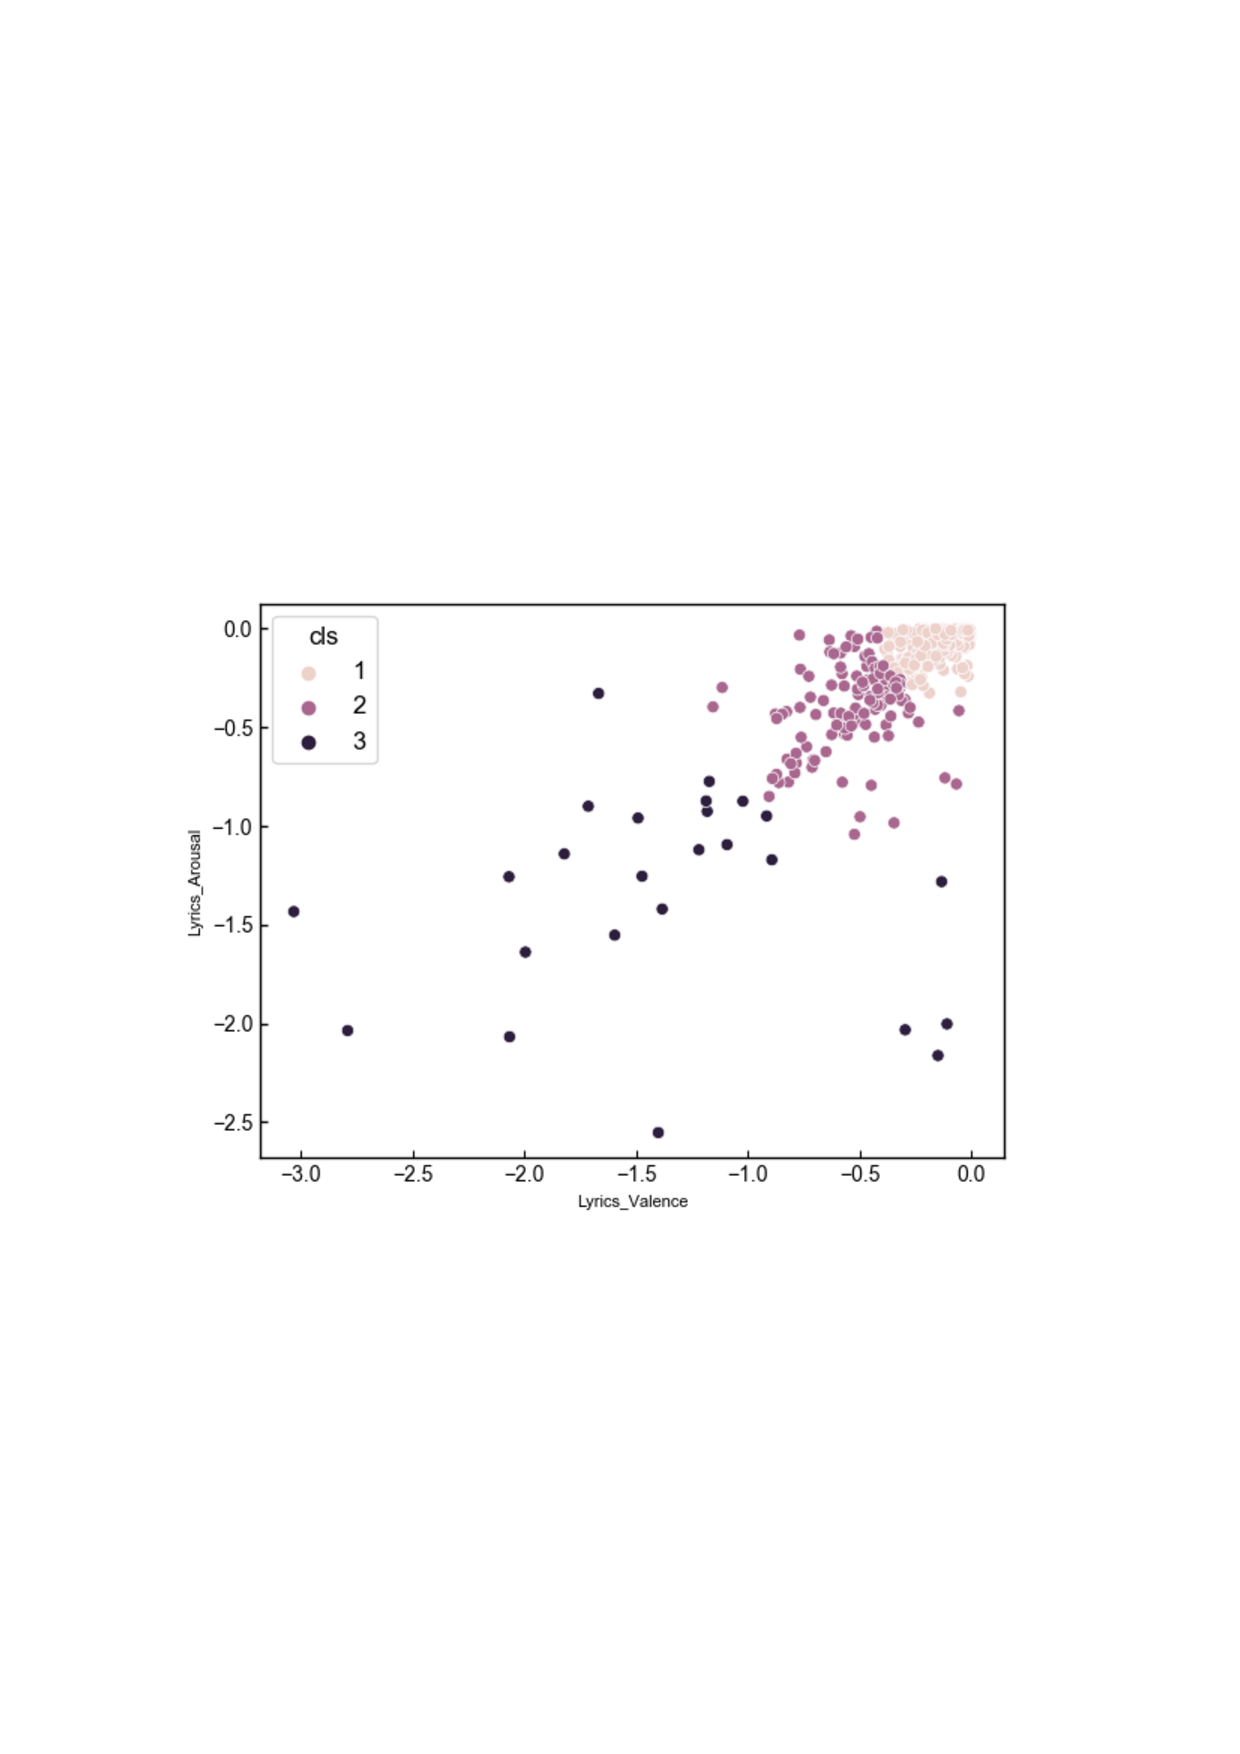
\includegraphics[width=14cm]{lyrics_A-V-.pdf}
  \vspace{-1mm}
  \caption{歌詞 A-V-平面}
  \label{fig:vkall}
  \vspace{5mm}
\end{figure}
第3象限にプロットされた楽曲は全部で388曲である.そのうちウォード法によって分割された曲数は第1グループが236曲,第2グループが127曲,第3グループが25曲であった.
後述する実験に用いる楽曲の歌詞データはそれぞれのグループからランダムで1曲分選出する.
第1グループからはEvery Little Thingの「Just be you」,第2グループからはコブクロの「コイン」,第3グループからはBUMP OF CHICKENの「分別奮闘記」の3曲を選出した.
\newpage
第4象限のプロット図は図3.6である.
\begin{figure}[H]
  \centering
  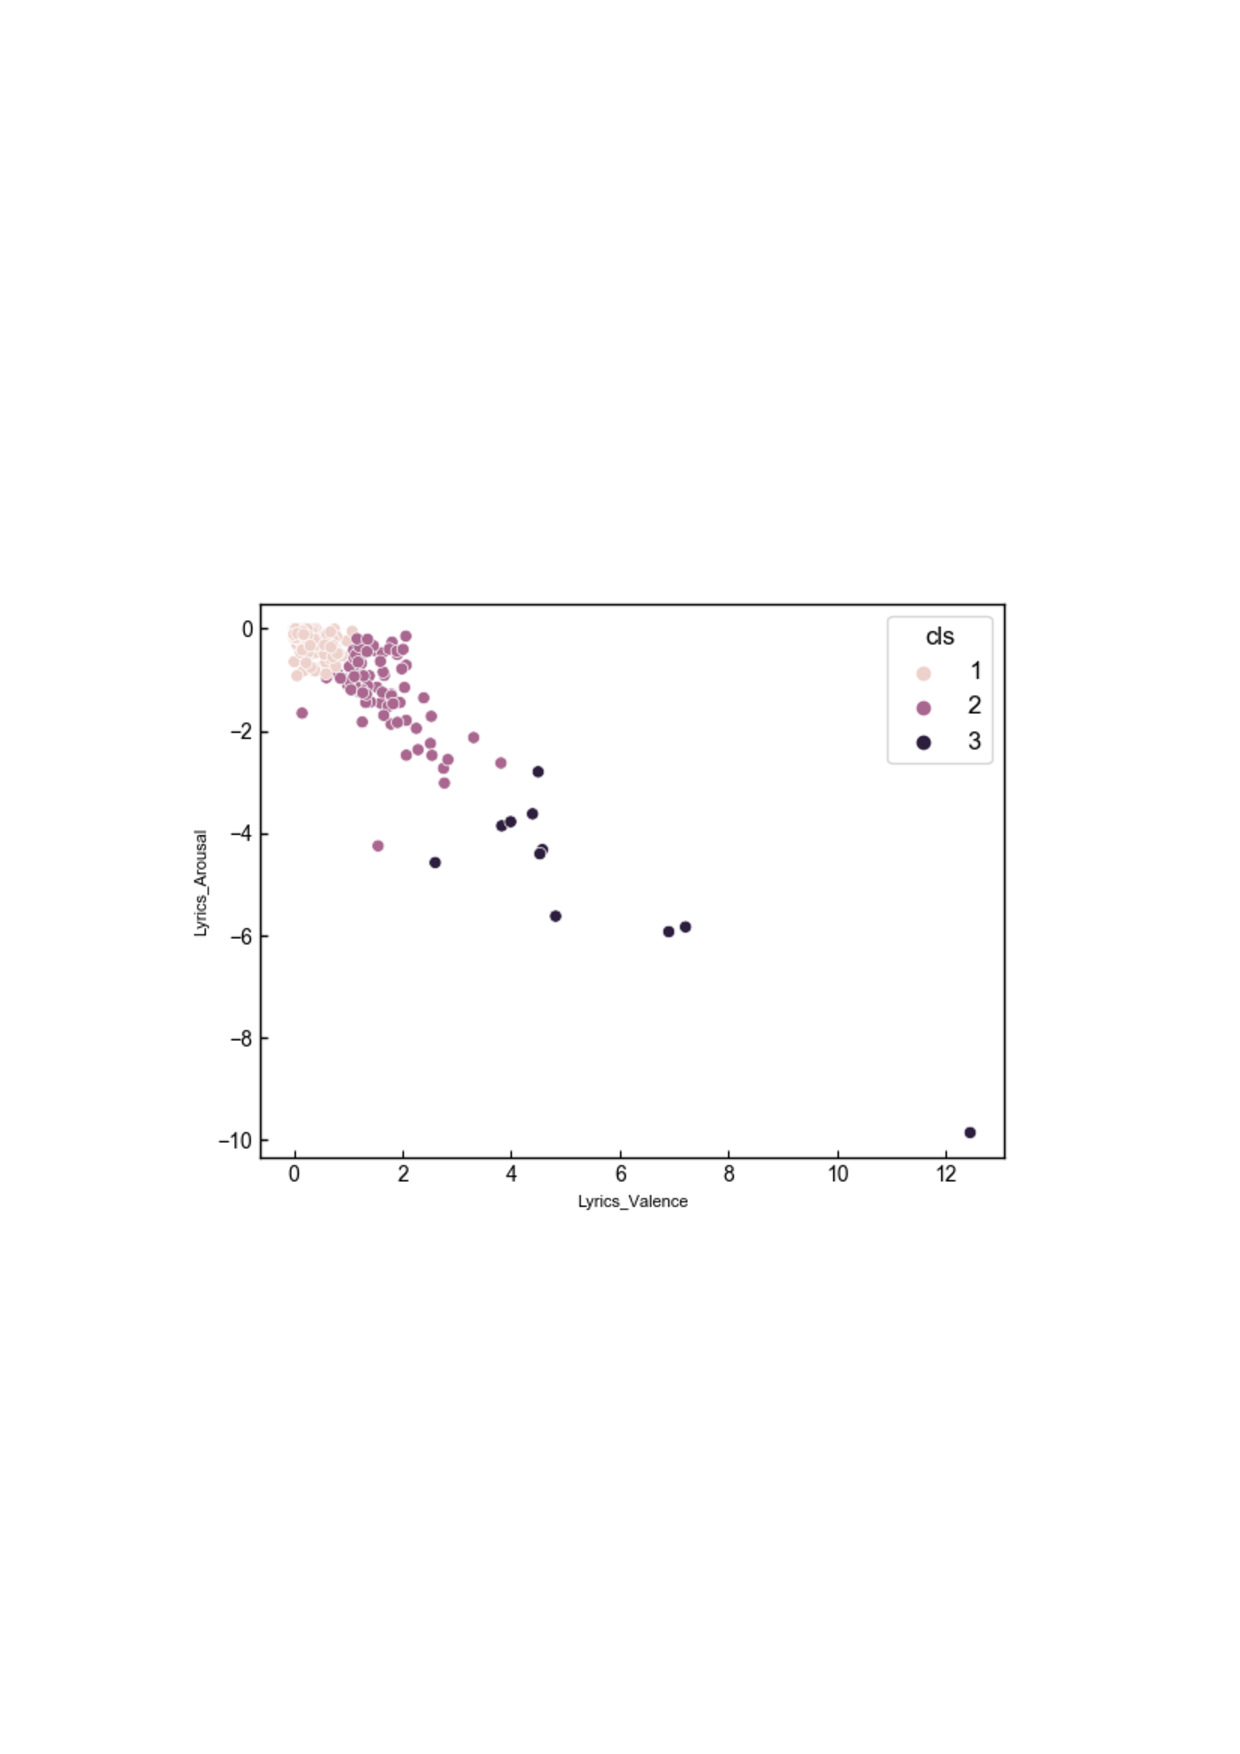
\includegraphics[width=14cm]{lyrics_A-V+.pdf}
  \vspace{-1mm}
  \caption{歌詞 A-V+平面}
  \label{fig:vkall}
  \vspace{5mm}
\end{figure}
第4象限にプロットされた楽曲は全部で302曲である.そのうちウォード法によって分割された曲数は第1グループが210曲,第2グループが81曲,第3グループが11曲であった.
後述する実験に用いる楽曲の歌詞データはそれぞれのグループからランダムで1曲分選出する.
第1グループからはUVERworldの「若さ故エンテレケイア」,第2グループからはあいみょんの「お互い様やん」,第3グループからはスピッツの「シロクマ」の3曲を選出した.
\newpage
\subsection{フレーズ}
歌詞に登場するフレーズをAV平面にプロットした.図3.7はAV平面に楽曲をプロットした図である.
\begin{figure}[H]
    \centering
    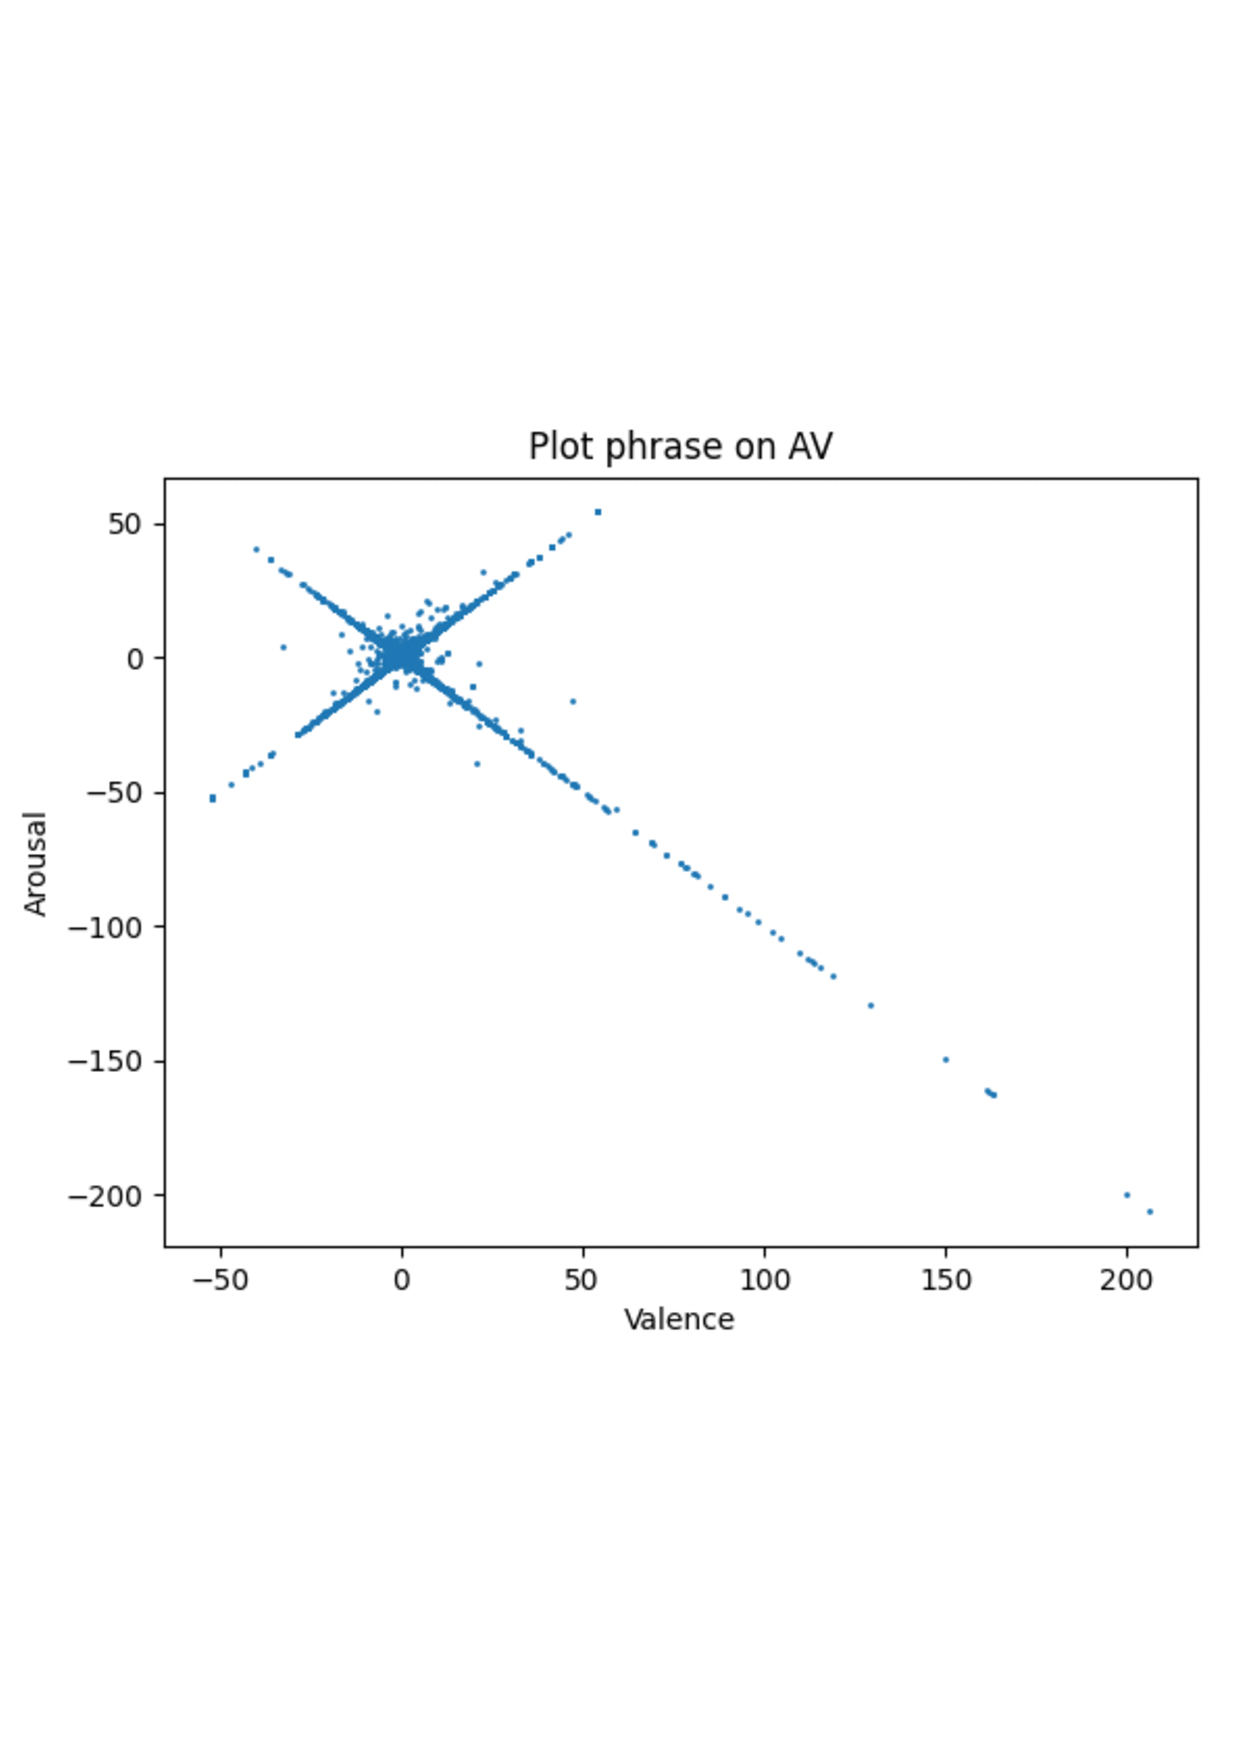
\includegraphics[width=12cm]{phrase_AV.pdf}
    \vspace{0mm}
    \caption{フレーズ AV平面}
    \label{fig:mms}
    \vspace{5mm}
\end{figure}
歌詞と同じく各印象ごとにフレーズを分類して,原点からの距離に基づいてward法でクラスタリングした.
\newpage
第1象限のプロット図は図3.8である
\begin{figure}[H]
    \centering
    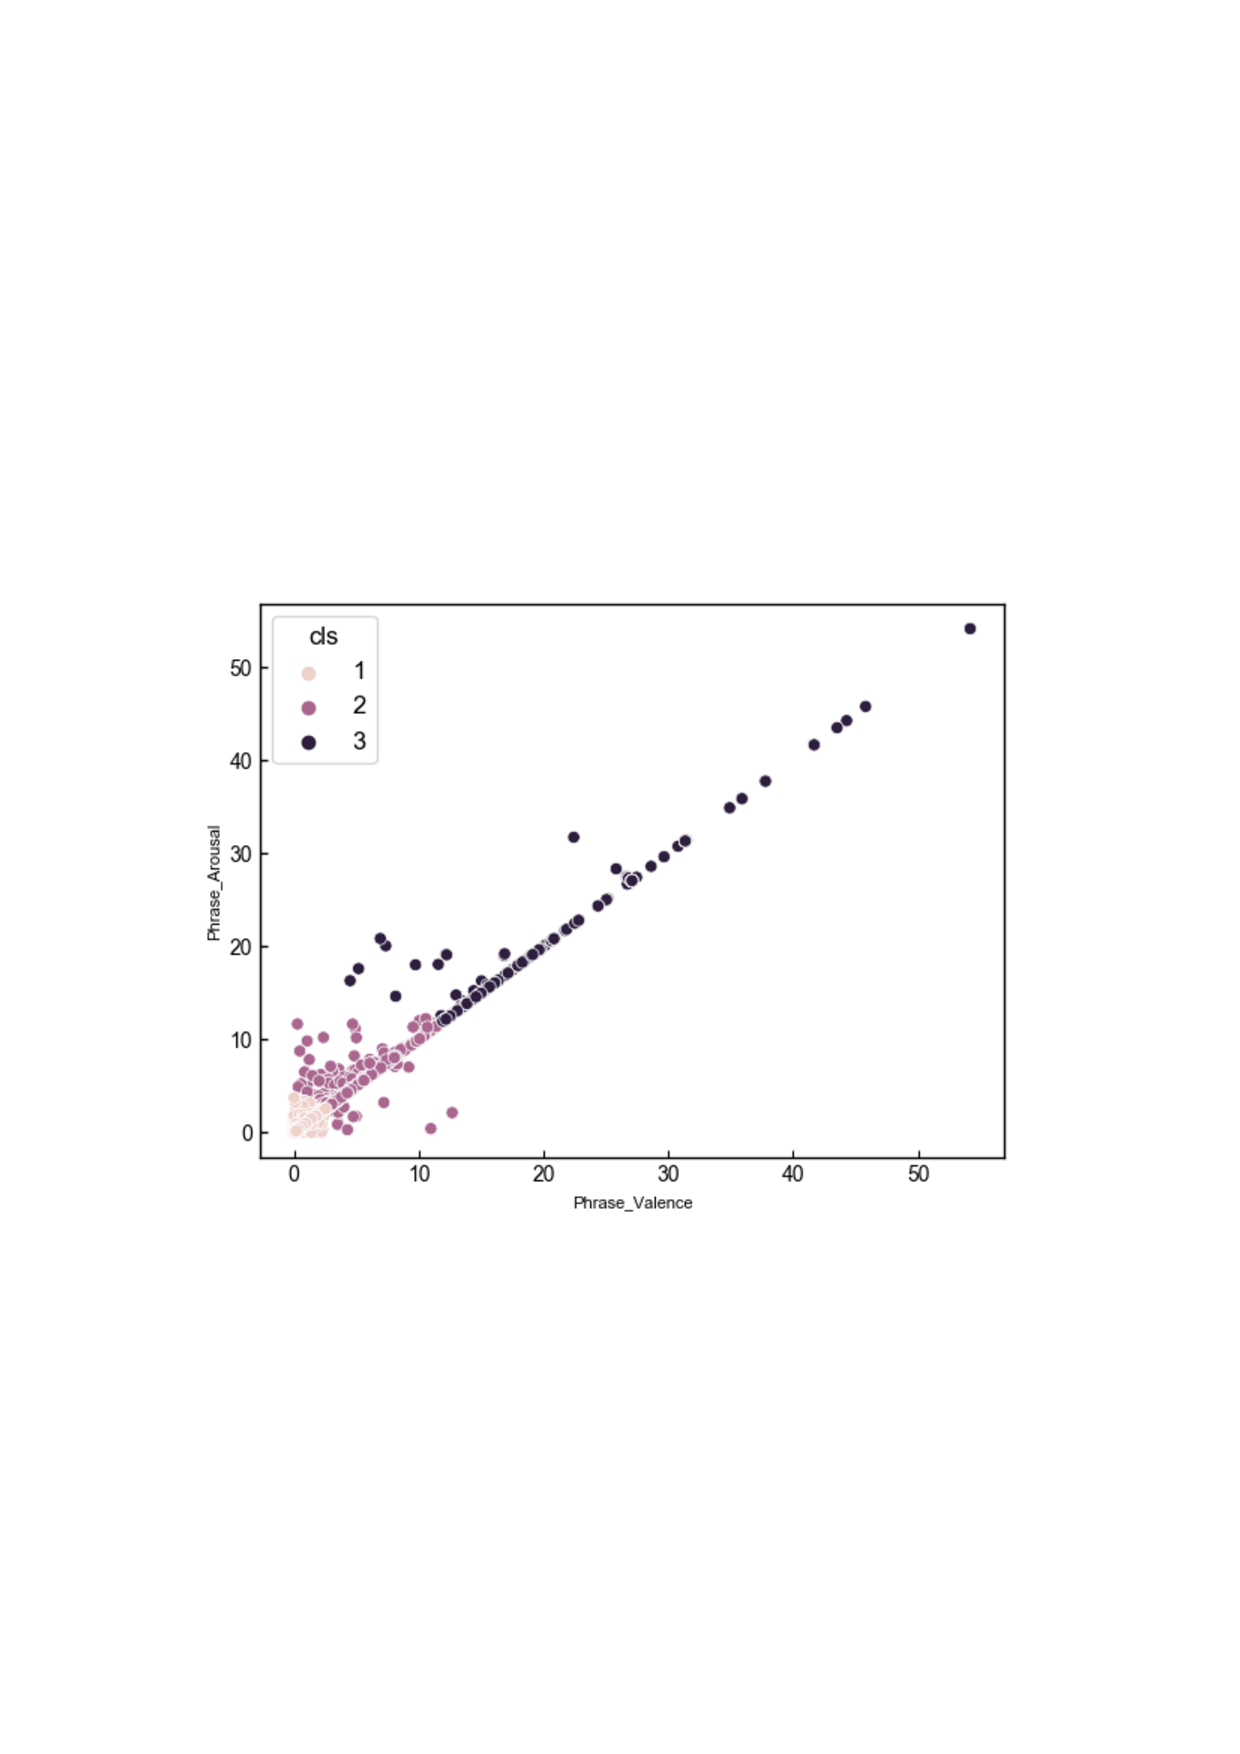
\includegraphics[width=14cm]{phrase_A+V+.pdf}
    \vspace{-1mm}
    \caption{フレーズ A+V+平面}
    \label{fig:mms}
    \vspace{5mm}
\end{figure}
第1象限にプロットされたフレーズは全部で35935句である.そのうちウォード法によって分割されたフレーズは第1グループが33,357句,第2グループが2,180句,第3グループが398句であった.
後述する実験に用いるフレーズのデータはそれぞれのグループからランダムで1句選出する.
第1グループからは「ひとりひとり違う世界みていくんだ」,第2グループからは「一石投じる生きる力」,第3グループからは「バタフライして」の3句を選出した.
\newpage
第2象限のプロット図は図3.9である.
\begin{figure}[H]
    \centering
    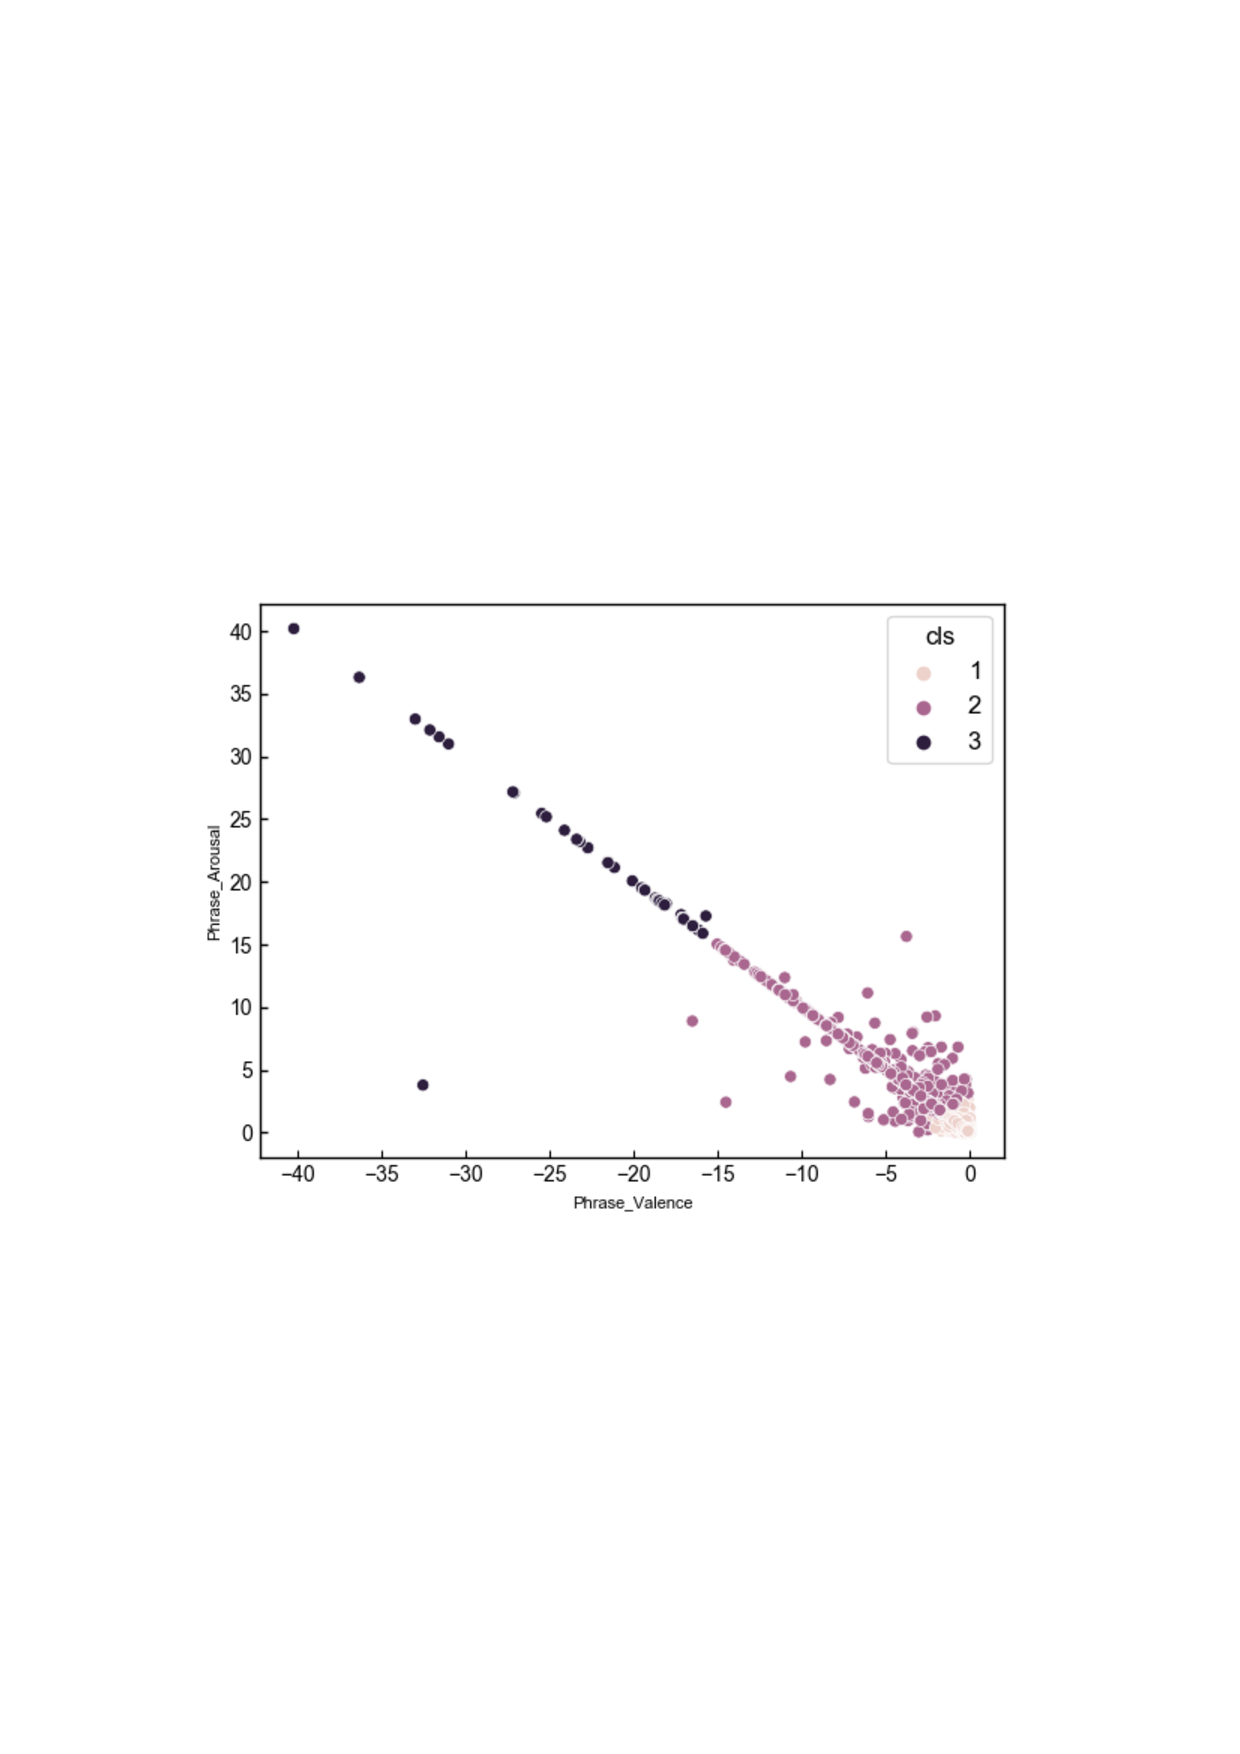
\includegraphics[width=14cm]{phrase_A+V-.pdf}
    \vspace{-1mm}
    \caption{フレーズ A+V-平面}
    \label{fig:mms}
    \vspace{5mm}
\end{figure}
第2象限にプロットされたフレーズは全部で27658句である.そのうちウォード法によって分割されたフレーズは第1グループが25,797句,第2グループが1,779句,第3グループが82句であった.
後述する実験に用いるフレーズのデータはそれぞれのグループからランダムで1句選出する.
第1グループからは「演じる意味はどこもブレたまま」,第2グループからは椎名林檎の「二つ並んだ影法師の手」,第3グループからはDREAM COME TRUEの「マイクホン争奪戦」の3句を選出した.
\newpage
第3象限のプロット図は図3.10である.
\begin{figure}[H]
    \centering
    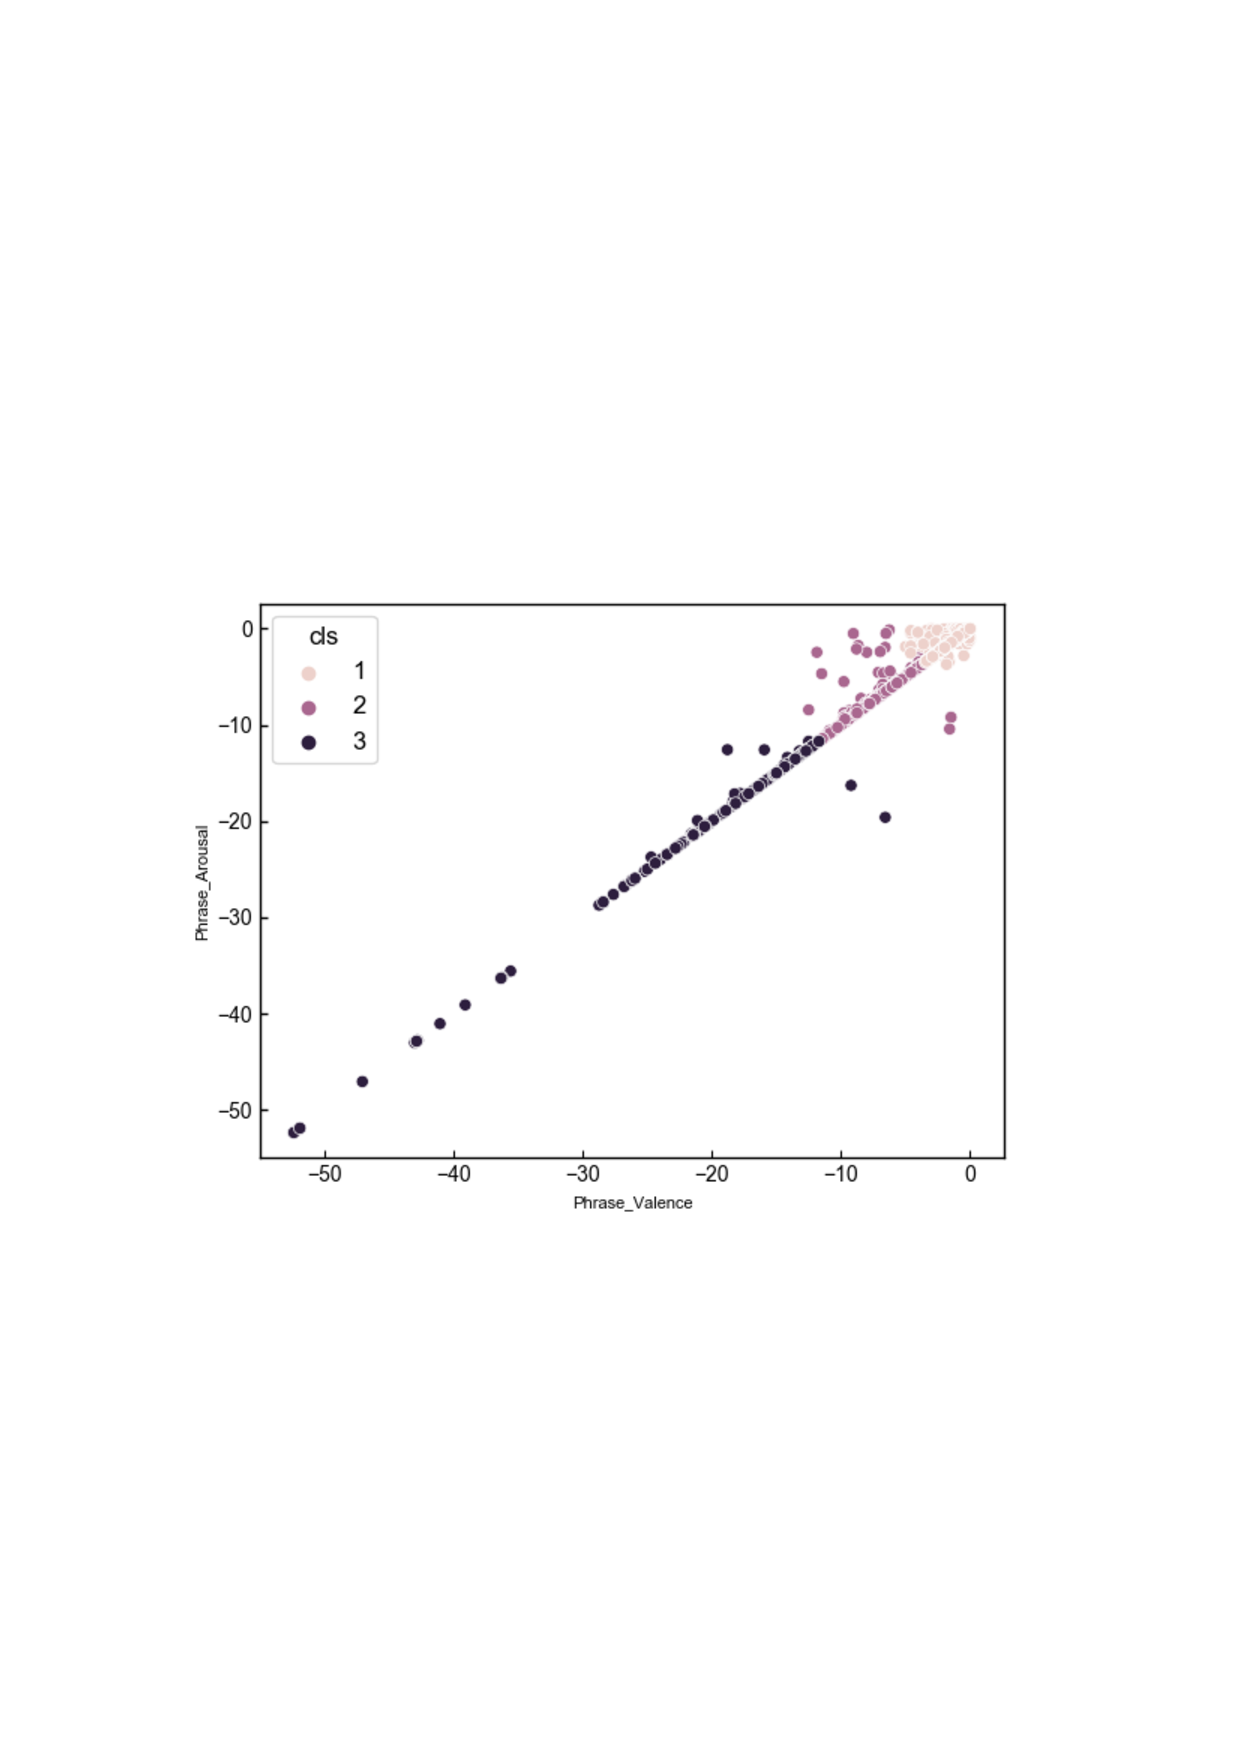
\includegraphics[width=14cm]{phrase_A-V-.pdf}
    \vspace{-1mm}
    \caption{フレーズ A-V-平面}
    \label{fig:mms}
    \vspace{5mm}
\end{figure}
第3象限にプロットされたフレーズは全部で14737句である.そのうちウォード法によって分割されたフレーズは第1グループが13,821句,第2グループが694句,第3グループが222句であった.
後述する実験に用いるフレーズのデータはそれぞれのグループからランダムで1句選出する.
第1グループからは「あたしを捨てたあなたは馬鹿で」,第2グループからは「あなたを苦しめたことでしょう」,第3グループからは「昨今のあなたは鼻につくわ」の3句を選出した.
\newpage
第4象限のプロット図は図3.11である.
\begin{figure}[H]
    \centering
    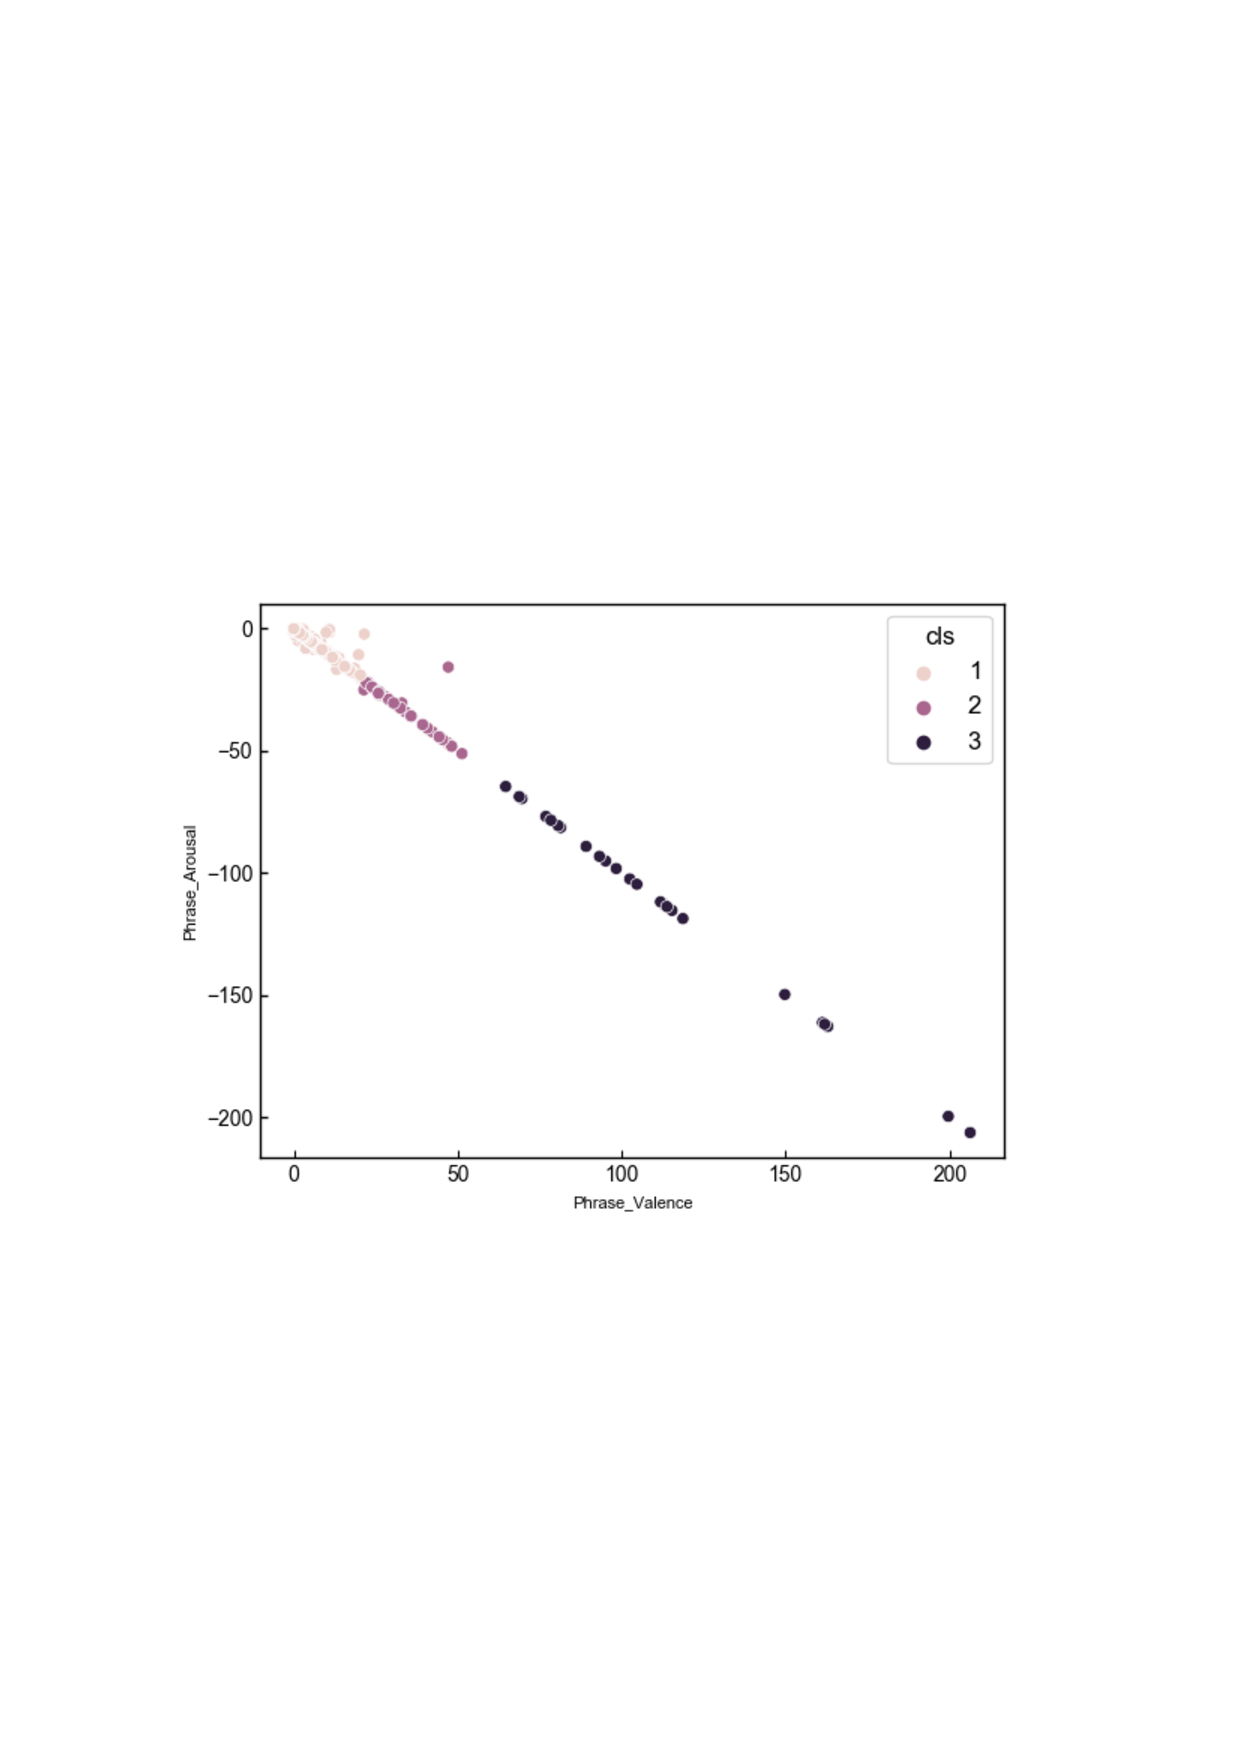
\includegraphics[width=14cm]{phrase_A-V+.pdf}
    \vspace{-1mm}
    \caption{フレーズ A-V+平面}
    \label{fig:mms}
    \vspace{5mm}
\end{figure}
第4象限にプロットされたフレーズは全部で60,000句以上である.第4象限にプロットされたフレーズ数は多かったので,重複削除をした後にランダムで30,000句を取り出した.そのうちウォード法によって分割されたフレーズは第1グループが29,907句,第2グループが64句,第3グループが29句であった.
後述する実験に用いるフレーズのデータはそれぞれのグループからランダムで1句選出する.
第1グループからは「浮かぶ月にやさしく響いては消えてった」,第2グループからは「染まる真っ赤なギロチン」,第3グループからは「しぶといトラウマも全部払おう」の3句を選出した.
